%# -*- coding: utf-8-unix -*-
% !TEX program = xelatex
% !TEX root = ../thesis.tex
% !TEX encoding = UTF-8 Unicode

\subsection{概述}
\label{sec:schema-intro}


以DBPedia、Freebase等为代表的开放领域知识库包含了
预先定义好的标准化的知识库谓词,
用于连接知识库中的实体、类型和概念。
知识库中的事实采用三元组形式表示,与关系三元组保持一致。
本节中,我们假定每个关系三元组均已完成了实体链接步骤,
用($e_{subj}$, $r$, $e_{obj}$)来表示。
那么很显然,事实三元组和关系三元组的区别仅体现在谓语成分上。
因此,利用知识库谓词来表示自然语言关系的语义,是一个很自然的想法,
若能将开放式信息抽取中的每一个关系实例都映射为知识库中的三元组,
那么机器将很容易理解海量非结构化文本中蕴含的结构化信息。
这种基于直接对应的思路非常直观,
但是对于现有的知识库,例如Freebase\cite{bollacker2008freebase},
即便其中包含十亿级别的事实三元组,
仍然会面临两个主要的挑战。

首先,知识库和自然语言关系之间存在着语义鸿沟。
以关系 ``has grandfather'' 为例,
Freebase中并不存在一个谓词能与之完全匹配,
但存在一些和它相关的谓词,例如\textit{parents}以及\textit{gender}。
这是因为知识库的构建过程较为严谨,为了避免歧义,每一种谓词的语义都更加单一,
同时为了避免信息冗余,能通过其它谓词进行描述的语义,通常不会对应一个单独的谓词。

其次,知识库的构建还远不够完整。
即便拥有海量的事实三元组,但依然存在很多长尾的谓词,并没有多少事实与之相关。
这个挑战也引入了另一个开放的研究课题,即知识库补全(Knowledge Base Completion)
\cite{gardner2015efficient,lao2010relational,lao2011random}。
该课题的目标是,给定知识库中的目标谓词,根据其拥有的少量事实三元组进行学习,
为其补充新的事实,这些新事实的主语和宾语均为知识库中已存在的实体。
换言之,在已有的实体之间连接更多的谓词,使知识库更加稠密。
%One natural research question is,
%is it possible to enrich the facts in an incomplete knowledge base by
%integrating massive relation instances discovered from Open IE
%\cite{gardner2015efficient,lao2010relational,lao2011random}.
%That is, given a triple (``Madelyn Dunham'', ``grandfather of'',
%``Barack Obama'') extracted from open domain text,
%if both entities already exist in the knowledge
%base as distinct nodes, but not yet connected, can we connect them
%using existing predicates?
%%This task is also known as knowledge base completion (KBC).
%Another related question is, can we translate a natural language
%query such as ``Who is the grandfather of Patrick Schwarzenegger?''
%into a structured query to the knowledge base, using,
%for example, SPARQL.
%This question is relevant to automatic question answering
%\cite{berant2013semantic,berant2014semantic,yao2014information,zou2014natural},
%a major challenge in natural language processing.
%These two challenges together form our research question:
%given a relation and a set of its instances discovered by Open IE,
%is it possible to add a corresponding predicate into KB,
%and populate this predicate based on existing knowledge?
%Answer to the question: represent new relation by
%existing structure knowledge rep.

%The answer to two challenges lies in the ability to
%learn a good knowledge base representation for a natural language
%relation, such as the one in \figref{fig:schema-intro}.



%TODO: \KQ{Compared with traditional KBC tasks ... }

%For example, Freebase doesn't have has-grand-father predicate,
%or even has-father predicate, but instead has the {\em parent}
%and {\em gender} predicates, which may jointly represent the semantics
%of has-grand-father (see \figref{fig:kb-schema}(b)).

%There are different ways to represent relations in a knowledge graph.
%Previous work
%\cite{gardner2015efficient,lao2011random,zou2014natural,zhang2012ontological}
%proposed to represent a relation by a {\em path} of
%predicates connecting the two entities in a knowledge base.
%Each node along the path is a variable entity of the type compatible
%with the predicates on either side of it. Such a path is
%called a {\em skeleton}.
%%along with discriminative
%%features on the edges and the nodes along the path.
%%\KZ{For example ...}.
%The advantages of such representation are
%i) it is intuitive; ii) it can be translated into
%SPARQL queries straightforwardly and hence all existing RDF tools
%can be used; and iii) it is human readable and allows manual fine-tuning
%if necessary.
%However, one limitation is that a path of predicates may not
%be accurate enough to represent a {\em complex} relation.
%For example, ``has grandfather'' relation could
%be represented by {\em parent} + {\em parent} path in Freebase,
%but this brings in additional noise since grandmothers are also included.

为了应对以上两个挑战,我们关注的重点在于
能否利用知识库中已经存在的谓词,描述一个自然语言关系所具有的语义。
已有的相关研究方法主要可以分为两大类。
第一类方法为知识库的向量表示学习。
%\cite{bordes2013translating,wang2014knowledge,guo2016jointly,wang2016text,nickel2015holographic}
这种方法类似于词向量技术,利用知识库中的三元组作为训练数据,
学习每个实体以及谓词在连续空间中的特征表示,
使得每个三元组的两个实体和谓词表示之间满足特定的代数关系。
%这类方法也称为基于翻译模型的的指示表示学习。
%\cite{bordes2013translating,wang2014knowledge,guo2016jointly,wang2016text,nickel2015holographic}
%\KQ{missing refs: HOLE, CPRA, AMIE+, and ``statistic schema induction'',
%since somehow I can't visit google scholar (either using proxy or not)}
%%(TransE, TransH, Hole, Guo), %Name + Citation
%\XS{refs fixed, re-check}
将开放式信息抽取的关系三元组与知识库已有的事实三元组合并,
这类方法可以获取每一个目标关系的隐含语义。
但考虑到知识库表示学习中涉及到的参数数量非常庞大,
这种方法需要大量的训练数据以应对长尾实体,同时训练的时间开销也不可忽略。
已有的研究工作主要集中在了较小的知识库上,
例如FB15K\cite{bordes2013translating,toutanova2015representing}。

%Moreover, due to large time and memory requrements in the training step,
%previous works only perform experiments on subsets of the knowledge base
%\cite{bordes2013translating,guo2016jointly},
%rather than the full version.

另一类方法为规则推导,每个目标谓词或关系的语义表达由明确的规则构建而成。
%\cite{lao2010relational,lao2011random,gardner2014incorporating,gardner2015efficient,wang2016knowledge,galarraga2013amie,galarraga2015fast}.
%(SFE, PRA, CPRA, AMIE+)
这里的规则等价于知识库的子结构,用于连接自然语言关系中的主语和宾语实体。
其中最基本的结构为路径的形式,即通过一个或多个谓词组成序列,
连接主语和宾语。
%TODO:讲的还不够清晰
规则推导方法的优势在于高度可解释性。
一方面,知识库的子结构可以转换为知识库上的查询语言例如SPARQL,
因此可以通过在知识库上运行查询的方式,
明确得知特定的两个实体之间是否可能存在某种关系。
另一方面,相比知识库向量学习方式,
基于规则推导的方法允许使用多条规则描述同一个关系,
更好地适应自然语言中的多义性。
此外,必要的情况下,人类可以对输出的规则进行微调。
%对于语义理解的下游应用来说xxxx。

%if necessary (for example, finding potential ambiguities in one relation).
%Because there are many possible rules in a given knowledge base,
%it's challenging to find the most effective rules.
%\KQ{Currently we don't talk about the others disadvantages of skeleton based method,
%since we will discuss the advantage of schemas in the later part of this section.}
%Another problem is that the selection of such features can be
%random and ad hoc.
%For example, {\em anyrel} is a feature that represents any predicate
%in the knowledge graph; the difference between the numerical values
%on two different nodes can be a feature as well. A more serious
%disadvantage is that such representation cannot be readily translated into
%SPARQL queries. Instead additional program code must be written to support
%queries, such as whether $e_1$ and $e_2$ has certain relation, or given
%$e_1$ and a relation, what is $e_2$. Finally, feature-based approach
%represents a relation by a bunch of weights, which are not human
%readable and are hard to explain.



根据以上论述,本节的研究建立在规则推导的基础之上。
%TODO: 为什么要使用schema,而不是path,用professor of和grand father举例子
%TODO: 这里绝对要补很多东西,而且没法在外面聊。
因此,我们将传统的基于路径的规则进行扩展,
而是以树形结构的形式,不仅连接主语和宾语,同时还连接了
其余相关实体,用于表示目标关系所具有的隐藏语义限制。
%根据前例可知,
这种树形结构是具有相同边结构的知识库中具体子图的抽象表示,
我们将其称为\textbf{模式图}(Schema Graph)。
\figref{fig:schema-intro}是二元关系 ``has grandfather'' 的模式图,
%类比数据库中的表格和视图
通过谓词路径[ $parents$, $parents$ ]表示主宾语之间的祖孙关系,
同时利用$gender$限制宾语的性别,以此精确描述关系语义。


%  In this paper, we propose to generalize the path structure
%  into a tree structure connecting not only the two target entities, but also
%  other constants and constraints connected to the path.
%  This tree structure is an abstraction of a set of all
%  concrete sub-trees in the knowledge base having the same edge
%  structure.
%  %Another perhaps more natural representation of a type of relation
%  %in a knowledge graph is a subgraph structure. This subgraph
%  %is an abstraction of all the concrete subgraphs of the same shape
%  %that connects each individual pair of the entities in the knowledge graph.
%  %This subgraph connects constant entities as well as variables.
%  We call such a tree structure a {\em schema graph}, or {\em schema}
%  in short.  \figref{fig:schema-intro} is an example schema graph,
%  which is essentially a view on the knowledge base,
%  joining several primitive predicates together.
%  %For example, the has-grand-parent relation can be represented by
%  %the Freebase schema shown in \figref{fig:kb-schema}(b), while
%  %the starring-in relation can be represented in \figref{fig:kb-schema}(c).

\begin{figure}[ht]
\centering
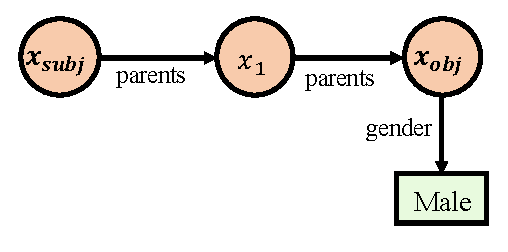
\includegraphics[width=0.4\columnwidth]{figure/schema/intro.eps}
\bicaption{二元关系 ``has grandfather'' 的语义表示。}{An example schema graph.}
\label{fig:schema-intro}
\end{figure}

具体而言,给定自然语言中的关系$r$以及抽取出的三元组$(e_{subj}, r, e_{obj})$,
本章的研究任务是在知识库中挖掘出一系列与之相关的模式图,
并且用概率分布的形式,描述用特定模式图代表该关系语义的可能性。
%The schema representation is formed in a tree structure, which
%consists of the predicate path connecting two entities directly,
%and constraint predicates at the branch of the path.
%Therefore, our paraphrasing task is the generalization of previous
%path-based work.
%This generalization is important because complex relations that
%require constraints constitute a non-trivial portion of
%all extracted relations from open IE.
%For example, by manual inspection, out of 2,500 most popular
%relation patterns in PATTY dataset,  13\% of the relation instances
%%and 7.5\% \KQ{18\% in our experiment} of relation patterns
%are actually complex (i.e., require more than a simple path to represent the semantics).
在进行模式图推理的过程中,我们主要会面临以下三个技术性挑战:

首先,候选模式图的数量非常庞大。
传统的规则推导中只考虑谓词路径,虽然候选路径的数量随长度呈指数增长,
但在知识库中能够连接两个特定实体的路径仅有少数,
因此简单遍历可以得到所有的候选路径。
然而,具有树形结构的模式图中,不仅存在额外的谓词作为分支,
而且包括用于语义限制的实体,任何一个实体的改变,都会产生一个新的模式图。
若使用暴力枚举生成模式图,时间复杂度上无法承受,
同时还会生成大量偏离语义的模式图。

其次,模式图推理需要做好粒度上的平衡。
当一个模式图缺少足够的语义限制,它虽然能匹配已知的三元组,但也可能混淆了错误的三元组。
反之,若一个模式图包含了不必要的语义限制,就很可能无法匹配已知的三元组。
很显然,太具体或宽泛的模式图都无法精确表示一个关系的语义,
但是如何兼顾这两点,并通过概率分布描述不同粒度候选的语义匹配程度,
这成为了模式图推理过程中的另一个难点。

最后,模式图推理模型仅有三元组作为训练数据,
不存在标注好的模式图,同时没有明确给出不符合特定关系的错误三元组数据,
这给学习过程增添了难度。
一种规避方法是使用封闭世界假设(Closed World Assumption),
即假定所有未见过的三元组都是错误的。
但考虑到知识库本身远不够完整,封闭世界假设会带来大量的错误反例,
这并不是一个最好的解决方案。

%In general, simpler schemas tend to be more general in meaning,
%whereas more complex schemas are more specific in meaning.
%A schema that is too general is less expressive and less informative,
%while a schema that is too specific may not be able to cover all
%the entity pairs.

%We define the notion \textbf{simple schema}, if the schema graph cotains \textit{only}
%a path of predicates connecting entities from $e_1$ to $e_2$ in the knowledge base.
%To this end, state-of-the-art systems have been proposed for solving this task.
%

%2. what's knowledge base try to do
%Structured knowledge base (KB) is a graph based taxonomy containing real world
%entities,  types,  binary predicates between entities and ``IsA'' relations
%between entities and types.
%(Machine readable, containing millions / billions of facts)

%Structured KBs such as WordNet \cite{miller1995wordnet},
%Yago \cite{suchanek2007WWW} and Freebase \cite{bollacker2008freebase} are widely used in information extraction
%and semantic learning tasks. In order to make relation schemas understood by human, we leverage types
%in the KB as the output of relation schemas.

%3. what to do is to extract schema
%The paraphrasing task is to map a natural language relation into structured
%canonical forms in KB, which is understood by both machine and human.
%
%We call the representation as \textit{relation schema} throughout this paper.
%
%\KQ{how to give a clear impression on schema}
%%\cite{bollacker2008freebase}
%%%Figure show schema on FB as the first impression (mention FB's size here)
%informal
%One can see that a relational schema is a template of many subgraphs
%with the concrete structure in the knowledge base.
%The goal of this paper is to enable effective and efficient translation
%process, which we call ``paraphrasing.''


%add. why we need to schema
%Paraphrasing is a open task, since the structured schema is an important knowledge
%used in many down-stream applications, such as question answering, text entailment
%and short text similarity querying.
%(Arguing)

%1. why we need paraphrasing

%2. what's the advantage of schema
% SPARQL query
% user intent query (check view synthesis paper)
%Paraphrasing is a fundamental task in natural language processing and understanding,
%especially in the system of question answering ,
%and knowledge base completion.
%In these tasks, the relation coming from input sentence (or question) is transformed
%into semantic structure in the knowledge base, and the overall accuracy is largely
%determined by the quality of the structural representation.
%
%
%There are three main advantages for our schema based model.
%First, each schema is an independent structure that represents the target relation.
%Feature weights produced by discriminative model can tell us which schemas are more
%suitable for the relation, while a single feature snippet is less expressive.
%Second, the schema is a subgraph of a semantic knowledge base.
%Our system can easily transform a schema into a SPARQL query due to the widely used RDF model
%in semantic knowledge bases. Therefore, an end-user can query RDF to retrive instances
%or a natural language relation, even though they don't know how to write a SPARQL query.
%Third, the schema is human-readable. Interactive online QA systems can display schemas and
%allow end-users to adjust them, leading to a better user experience.
%
%

%4. claim the gap between kb and nl on description
%Recap the semantic gap between relations and knowledge base predicates that we mentioned
%Yet some knowledge base is lack of predicates, however, the gap couldn't be removed,
%even for Freebase containing thousands of binary predicates.
%%5. simple exmple & chain example (mediator)
%%6. branching example
%%a) place_of_birth v.s. <people, was born in, place>
%%b) mediator: film.actor.film --> film.performance.film   v.s.   "starring in"
%%c) branching: female spouse v.s. "wife of"
%The predicate name ``place\_of\_birth'' in \figref{fig:fb-schema} (a) shows the difference,
%compared with relation words ``was born in'';
%\figref{fig:fb-schema} (b) brings the gap to structural level, where the schema shows a
%complex ``parent + parent + male'' style, even ``grandfather'' relation is so common in
%the real world; Meanwhile, \figref{fig:fb-schema} (c) show that the schema must include
%a intermediate node (used to maintain the ternary relation ``actor plays a character in a film'').
%These varieties make the paraphrase task challenging.
%
%%traditional method & limits
%%0. informally, composite relation
%%(Lei Zou) (EMNLP 2011) (AAAI 2012) (Tran 2009) (EMNLP 2015)
%For the part of feature based supervised systems, the first branch is graph-walk based
%\cite{lao2010relational,lao2011random}, a candidate schema is drawn from the predicate path
%between some entity pairs, and the probabilistic distribution of random walking from $e_1$
%to $e_2$ in KB on the schema is used as a feature to train the importance of each path.
%The second branch is logic based \cite{zhang2012ontological}, where the system uses hand
%crafted soft rules to mine various features that leads to good relation schemas.
%Since soft rules are fixed and independent of relations, the dimension of feature space
%is limited.
%
%Besides, unsupervised models are also used. Zou et al. \cite{zou2014natural}
%followed the idea of TF-IDF score \cite{blabla} to calculate the best schema with respect to a
%speicifc relation. While different input relations could have overlap meaning, this situation
%causes a lower score of schemas representing the overlapping part.
%
%In addition, among all different paraphrasing solvers, the process of candidate schema
%searching could always be a big challenge. All systems discussed above only generate
%simple schemas (predicate paths), which is also a limitation for searching more
%specific and meaningful schemas.
%
% our approach
%1. IMPORTANT data-driven

%TODO:我觉得这里要加一段,可以稍微提到approach里面的东西,总之就是为了应对xxx,我们xxx。
%不是bullet的形式。
%啥是LP,TC,啥是高效剪枝,啥是具体的生成模型,这些都可以写啊!!!!!!

本章提出的基于模式图的规则推导模型旨在解决应对以上三个挑战,
其主要贡献可以分为以下四个部分:
\begin{enumerate}
\item{我们定义了自然语言关系的模式图。
和传统规则推导模型相比,模式图是谓词路径形式的规则扩展,
通过挖掘隐藏的关联实体,在路径之上构建分支,
准确描述关系的复杂语义;}
%(\secref{sec:schema-problem});}
\item{我们提出了一种基于局部搜索的启发式方法,通过高效的剪枝策略,
快速生成关系所对应的候选模式图;}
%(\secref{sec:schema-candgen});}
\item{我们提出了一种基于数据驱动的方法,将模式推理问题转化为
查询任务进行建模,并在不明确生成负面训练数据的情况下,
学习候选模式图之间的概率分布,实现不同粒度模式图的统一比较;}
%(\secref{sec:schema-inference});}
\item{我们对自然语言关系以及知识库中已有的谓词进行了知识库补全任务的测评,
包括主宾语预测和三元组分类两个子任务,
我们的模型在这两个测评任务上均显著优于已有方法。
具体生成的模式图结果表明,我们提出的模型能够挖掘出具体且精确的语义。}
%(\secref{sec:schema-exp})。}
\end{enumerate}


%  This paper addresses these challenges and makes the following contributions.
%  %We present a distant-supervised learning approach to solve the
%  %paraphrasing problem, with the following contributions:
%  \begin{itemize}
%  \itemsep0em
%  \item We define schemas as a generalized representation of natural language
%  relations in knowledge base (\secref{sec:problem});
%  \item %Due to the prohibitive space of possible schemas,
%  We present an effective local search based heuristic to generate a set of
%  candidate schemas (\secref{sec:candgen});
%  \item We propose a data-driven approach to model the schema inference
%  problem as a querying task, and thus compute the probability distribution over schemas,
%  given a natural language relation and its instances
%  without explicitly generating negative training data (\secref{sec:schema});
%  \item The framework significantly outperforms
%  previous best approaches on link prediction and triple classification task.
%  The example results show that our schema inference model
%  is able to discover concrete and precise semantics (\secref{sec:eval}).
%  %and question answering. Furthermore, our schema representation is
%  %on par with the popular word embedding model in computing relation similarity (\secref{sec:eval}).
%  \end{itemize}

